\chapter{Control Network Toolkit}
\label{ch:controlnettk}

This chapter covers the first additional boost of tools for \ac{ASP}!
Control Networks are a data structure that at their core contain image
features that can be tracked in multiple images. Since these features
can be tracked in multiple images, they can be triangulated and
represent a 3D location. This control network can then be used in
processes such as Bundle Adjustment using tools like
\texttt{isis\_adjust} and \texttt{jigsaw}.

\emph{Warning: This toolkit is not finished but this documentation
  hopes to allow some use in its early state.}

The method of developing a control network with \ac{VW} and \ac{ASP}
is that we try to track as many 'natural' features and then reduce
into a control network. This is done in a 6 step process.

\begin{itemize}
\item Detect features using a second order filter \emph{(LoG)}.
\item Describe these features by their surroundings with a tag.
\item Match tags of interest points between images.
\item Filter these matches for error using RANSAC.
\item Reduce matches further for ease of processing and also to assure uniform distribution.
\item Collect all pair-wise matches and write as Control Network.
\end{itemize}

I'm going to provide an example of how to use this software with
Apollo Metric images. Hopefully you can follow along with whatever
imagery you happen to have around. Note in the example below we use a
lot of calls to \texttt{xargs}. That command is helpful for spawning
multiple processes to work on a pool of jobs. The argument \emph{\-P 10}
states that at most it should have 10 processes running
simultaneously. Lower that value to the number of cores available on
your system.

We are going to start out first by gathering interest points \emph{(or
  features)} and this is accomplished with a tool called
\texttt{ipfind}. This handy tool is provided by \ac{VW} and is not
built against ISIS. This means it can only read cube files through a
library called GDAL. To make sure cubes files can be read correctly by
GDAL and thus ipfind, we'll have to convert our input imagery to
something more reliable like TIFFs.

\begin{verbatim}
    ISIS 3> isis2std from=INPUT to=OUTPUT.tif format=TIFF
\end{verbatim}

I don't like to call isis2std on every file myself. Here's the
commands I use to do this in parallel.

\begin{verbatim}
    ISIS 3> echo *.cub | xargs -n1 echo | awk -F "." '{print $1}' |
              xargs -n1 -P 10 -I {} isis2std from={}.cub to={}.tif format=TIFF
\end{verbatim}

The directory should now be filled with TIFF format doppelgangers. We
are ready to perform \texttt{ipfind} which will detect features and
describe them in one go. The results of each operation will be saved
in a \texttt{.vwip} file which will later be read during
matching. There are many algorithms that \texttt{ipfind} can use for
detection and description but the defaults of OBALoG and SGrad should
do fine for most situations. Also note that \texttt{ipfind} has a
debug flag '-d' which can be used to output debug images that show the
location of all detected features.

\begin{verbatim}
  > echo *.tif | xargs -n1 -P 10 ipfind --max 10000
\end{verbatim}

Notice the options \emph{\-\-max 10000} used for the \texttt{ipfind}
example. This is to limit the number of detected interest points so
that the next step doesn't take too long.

Matching is calculated pairwise. There are many ways to do this, but
the simplists is just a brute force permutation of all possible
combinations. Here's how:

\begin{verbatim}
  > pairlist_all.py *.tif | xargs -n2 -P 10 ipmatch -r homography
\end{verbatim}

Alternatively we could just match between images that happen to be
sequential by name.

\begin{verbatim}
  > pairlist_seq.py *.tif | xargs -n2 -P 10 ipmatch -r homography
\end{verbatim}

Though for large datasets it doesn't seem approriate to compare all
images to each other as the physically don't see each other in
anyway. A good way of reducing the matches is by deciding to only
calculate matches between images that are separated by no more than a
few degrees. This is what \texttt{pairlist\_degree.py} can
do. Internally it calls \texttt{camrange} and this can take a
while. I'd recommend saving the output to a file before sending out to
ipmatch.

\begin{verbatim}
    ISIS 3> pairlist_degree.py *cub -a 10 -iext tif > pairs_to_process.lst
    ISIS 3> cat pairs_to_process.lst |
              xargs -n2 -P 10 ipmatch -r homography
\end{verbatim}

If you've been reading the output from ipmatch, you may have noticed
that some pair-wise matches might have more than a 100 matches! This
is probably overkill for some cases and could potentially choke an
application further down the process. Also at this point, our interest
points could be located anywhere. The worst case is that all matched
features have managed to clump around interesting objects like a
sparkly crater or a sharp cut rill. We can't enforce that the matched
features are evenly placed, but we can trim them down to be somewhat
even.

Enter stage left, \texttt{reduce\_match}. This utility will thin down
the matches so that they are evenly distributed. You specify the
minimum and maximum amount of matches that can exist for a pair of
images. Setting the maximum trims down excessive matches. The minimum
however will actually delete match files that have to few matches. The
filtering function RANSAC that is used to remove outliers does not
have a graceful failure. When that algorithm fails it will return all
outliers but usually with the minimum number of matches to solve for
its fitting functor. Using a homography fitting functor means 8
matches. We'll go ahead and delete anything 10 and under.

\begin{verbatim}
  > echo *.match | xargs -n1 -P 10 reduce_match --min 10 --max 100
\end{verbatim}

Finally we are ready to collect all pairwise matches into a single
control network. From the same directory that houses all match files
and cube files, we will call the command
\texttt{cnet\_build}. Assuming we want to build an ISIS style control
network, here's how to perform the last step.

\begin{verbatim}
  > cnet_build *.cub -t isis -o asp_control
\end{verbatim}

Let's go ahead and see how the results turned out in qnet!

\begin{verbatim}
    ISIS 3> echo *.cub | xargs -n1 echo > cube.lst
    ISIS 3> qnet
\end{verbatim}

Inside qnet you'll want to click 'open'. On the first dialog you'll
pick out the \emph{cube.lst} file we just created. On the second, we
pick our created control network \emph{asp\_control.net}.

\begin{center}
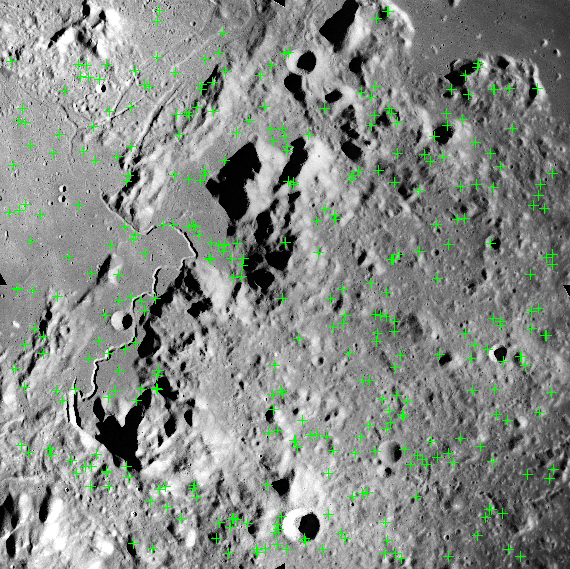
\includegraphics[height=3.7in]{images/cnettk_qnet_screen.png}
\end{center}

Occasionally you might find yourself not quite satisfied with results
of Control Network Toolkit. Don't worry, we won't take it
personally. However there are still some options available to you. You
could do manual tie point additions with \texttt{qnet}. However, this
can be a slow and scary process if you need to load up the entire
control network. Instead you can just load up the problem images and
do manual tie pointing. Then afterwards you could merge this smaller
control network with the large control network you created with
\texttt{cnet\_merge}.

\begin{verbatim}
  > cnet_merge large.cnet small.net -o larger.cnet
\end{verbatim}

The above command will create an even larger control network which
contains both \emph{large.cnet} and \emph{small.net}. This is helpful
for filling in those spots where the automatic control network failed
to work.
